\documentclass[twocolumn, 9pt,fleqn]{jsproceedings}

\interfootnotelinepenalty=10000

\renewcommand\refname{References}

\title{Image Stream Synchronization for Visual Navigation}

\author{Helio Perroni Filho (Doctorate Course, 2nd year)\authorrefmark{1}}

\affiliation{Intelligent Robotics Laboratory, OHYA's group}

\abstract{
Appearance-based navigation methods commonly require pairing up images from two separate sequences -- a reference \textit{teach step} record and the record of the current \textit{replay step} -- in terms of viewpoint proximity. This task is complicated by environmental variations such as lighting changes, viewer pose differences, moving objects and landmark occlusion. This article presents an image similarity metric, \textit{feature point correlation}, which is shown to behave well under such conditions.
}

\keywords{Image Processing, Machine Learning, Navigation}

\begin{document}
\thispagestyle{myheadings}
\markright{2014年度 第2回 山彦シンポジウム [2014/11/29--11/30 つくば研究支援センター,つくば国際会議場]}
\maketitle

\authorreftext{1}{Graduate School of Systems and Information Engineering,\\ University of Tsukuba}

\section{Introduction}

\textit{Appearance-based navigation} is a robot navigation paradigm where the environment is represented as image sequences collected along a route, which are matched to live sensory input in order to estimate current robot pose~\cite{BON02}. In comparison to Visual SLAM methods~\cite{AUL08}, it constitutes a less computationally expensive, more intuitive model, closer to how humans navigate our surroundings. The typical appearance-based navigation use case is \textit{teach-replay}, where a robot is led through an environment by a guide (the teach step), and must then autonomously retrace the original path, orienting itself by the data gathered during the guided phase (the replay step)~\cite{BUR01}. Figure~\ref{fig:teach_replay} illustrates the concept.

\begin{figure}[h!]
\vspace{20pt}
\includegraphics[width=\columnwidth]{teach_replay.pdf}
\vspace{10pt}
\caption{Teach-replay navigation use case. A mobile robot is first taken along a path by a guide (a), and must later retrace it autonomously (b).}
\label{fig:teach_replay}
\end{figure}

Appearance-based navigation methods commonly require pairing up teach and replay images by viewpoint proximity. Formally, let the image sequence collected over the teach step and the image sequence collected so far over an ongoing replay step be represented respectively by:
\begin{alignat}{3}
& S_{teach} & = & [I_1, \dotsc, I_i, \dotsc, I_m] \\
& S_{replay} & = & [I'_1, \dotsc, I'_j, \dotsc, I'_n]
\end{alignat}

The robot's pose at the time an image $I$ was taken is given by the \textit{viewpoint function}:
\begin{equation}
o(I) = (x, y, \theta)
\end{equation}

The \textit{pairing function} $g(I'_j)$ is defined over the domain of replay step images such that  $g(I'_j) = I_i$ is the teach image whose corresponding viewpoint $o(I_i)$ is the most similar to the viewpoint $o(I'_j)$ of replay image $I'_j$:
\begin{equation}
g(I'_j) = \arg \min_{I_i \in S_{teach}} {\|o(I_i) - o(I'_j)\|}
\end{equation}

Obviously if $o(I)$ were reliably known at any one time there would be no need for image pairing in the first place. Therefore what is needed is an approximation $g'(I'_j)$ that circumvents this requirement. In particular, \textit{appearance-based pairing} methods exploit the insight that changes to robot pose cause predictable changes to visual input, and therefore it must be possible to design an image similarity metric that correlates well to pose proximity~\cite{HEL13b}. Table~\ref{tab:methods} relates a number of such methods proposed in the literature.

\begin{table}[t]
\centering
\caption{Summary of appearance-based image pairing methods proposed in the literature, characterized in terms of employed sensors, test environments, and variations allowed between teach and replay steps.}
\renewcommand{\arraystretch}{1.5}
\setlength{\tabcolsep}{5pt}
\tiny
\begin{tabular}{|m{2.2cm}|m{1.4cm}|m{0.7cm}|c|c|c|}
\hline
    \multirow{2}{*}{\centering Method} & \multirow{2}{*}{Sensors} & \multirow{2}{*}{Tested} & \multicolumn{3}{|c|}{Landscape Variations} \\
\cline{4-6}
    & & & Lighting & Occlusion & Movement \\
\hline
    \mbox{Minimal template matching} \mbox{error~\cite{MAT96}} & Monocular camera & Indoors & No & No & No \\
\hline
    \mbox{Cost function} \mbox{minimization~\cite{OYA96}} & Monocular camera & Indoors & No & No & No \\
\hline
    \mbox{Mutual information~\cite{STE12}} & Monocular camera & Indoors & No & Yes & Yes \\
\hline
    Feature point tracking~\cite{CHE06} & Monocular camera & Indoors, Outdoors & Yes & No & Yes \\
\hline
    \mbox{Local best match and} \mbox{sequence recognition~\cite{MIL12}} & Monocular camera & Outdoors & Yes & Yes & Yes \\
\hline
    \mbox{Stereo feature matching and} \mbox{visual motion estimation~\cite{KIM08}} & Stereo camera & Indoors & Yes & Yes & Yes \\
\hline
    Average Landmark Vector~\cite{LAM00} & $360^o$ panoramic camera, polarized light sensor, wheel encoders & Simulation, Outdoors & Yes & No & No \\
\hline
    \mbox{Block matching} \mbox{Optical Flow~\cite{VAR05}} & $360^o$ panoramic camera, wheel encoders & Indoors & Yes & Yes & No \\
\hline
\end{tabular}
\label{tab:methods}
\end{table}

This article describes the \textit{feature point correlation} appearance-based pairing method, designed to work well under both natural and artificial lighting conditions, and also against changes in lighting, landmark occlusion and moving objects. The article's remaining sections are organized as follows: first, related works are presented in terms of proposed image pairing methods. Next feature point correlation is described, followed by experiments demonstrating its performance. Directions for further research are discussed in the conclusion.

\section{Related Work}

Image pairing methods based on cost minimization define a mismatch metric between any two images, then pair up replay images to least mismatched teach images. Template matching~\cite{MAT96} is a straightforward way to implement this. A more involved alternative, noted for its resource efficiency~\cite{BON02} is to extract vertical lines from teach and replay images, then define mismatch in terms of differences in intensity, position and number of lines in each set~\cite{OYA96}. However, these metrics are vulnerable to changes in lighting, landscape appearance and the presence of moving objects, having been successfully tested only in static indoors environments. Mismatch metrics in general are also susceptible to ambiguities in environments with many repeating features, such as long corridors.

Mutual information~\cite{STE12} and Kanade-Lucas-Tomasi (KLT) feature tracking~\cite{CHE06} have been proposed as more robust mismatch metrics. Ambiguities over repeating environmental features can be resolved by splitting teach records in segments delimited by milestone frames, and then limiting the search to a single segment at a time. The transition from one segment to the next can be determined by watching the intensity of the mismatch between current input and the next milestone: a reversal from a decreasing to an increasing trend indicates the milestone has been passed~\cite{MAT96,CHE06}.

Another way to make mismatch minimization more robust is to look not for a global best match for each visual input, but instead to look for coherent sequences of ``good'' matches between successive replay inputs and the teach record~\cite{MIL12}. Tested on video clips recorded from manually driven cars, this method was highly successful in recognizing revisited locations over a wide range of variations (day, night, rain, moving cars, seasonal changes, etc), but no tests involving actual autonomous navigation were performed, and test landscapes were restricted to open outdoors spaces.

Stereo vision systems can also use the KLT tracker to find correspondences between feature points in three-dimensional space. This method is less vulnerable to ambiguities in appearance, though it must still be complemented by motion estimation for cases where feature matching is not possible (e.g. due to the presence of moving elements or changes to the landscape)~\cite{KIM08}. This method was shown to reliably retrace paths as long as $60m$, but no results on lighting changes or outdoor tests have been reported.

Finally, panoramic cameras make possible to use methods that compare current visual input and stored images to compute \textit{direction vectors} pointing towards a target pose~\cite{LAM00,VAR05}. In this way the need for image pairing is sidestepped. However those methods require that a common landmark set remain visible throughout both teach and replay steps, limiting applicable range as well as robustness to landscape changes. Additionally, ensuring the panoramic camera will have a clear field of view all around the robot might be problematic from an engineering perspective, depending on form-factor considerations and application scenarios.

\section{Method}

\begin{figure}[t]
\includegraphics[width=\columnwidth]{pipeline.pdf}
\caption{Image pairing using the feature point correlation method. Image sequences recorded during teach and replay steps (a) are transformed by a mapping function (b) into respective teach and replay map sequences (c). Replay maps are dispatched to a feature extractor (d) which generates lists of feature points (e). The feature points along with teach and replay maps are dispatched to a patch extractor (f) which produces lists of patches from both the teach and replay map sequences (g). Patch correlation (h) is performed over these lists to produce a similarity map (i). A line-fitting algorithm (j) is executed over the similarity map to optimize the image pairing parameters (k), which are passed to the image sorter (l) along with the original teach and replay image sequences to assemble the sequence of image pairs (m).}
\label{fig:pipeline}
\end{figure}

Figure~\ref{fig:pipeline} provides an schematic overview of the feature point correlation method. The remainder of this section is dedicated to explaining each step of the procedure in detail.

As stated before, let the image sequence collected over the teach step and the image sequence collected so far over an ongoing replay step be represented respectively by:

\begin{alignat}{3}
& S_{teach} & = & [I_1, \dotsc, I_i, \dotsc, I_m] \notag \\
& S_{replay} & = & [I'_1, \dotsc, I'_j, \dotsc, I'_n] \notag
\end{alignat}

First, a mapping function $\eta(I) = H$ is applied to each image $I$ in the teach and replay sequences, producing a \textit{map} $H$ less susceptible to lighting variations:
\begin{alignat}{3}
& Z_{teach} & = & [H_i \; | \; H_i = \eta(I_i)] \\
& Z_{replay} & = & [H'_j \; | \; H'_j = \eta(I'_j)]
\end{alignat}

From each replay map a list of \textit{feature points} is extracted according to some definition of ``feature'':
\begin{equation}
P(H'_j) = [p_{j,1}, \dotsc, p_{j,k}, \dotsc, p_{j,z}]
\end{equation}

Where $p_{j,k} = (u_{j,k}, v_{j,k})$ is a point in map coordinates. Feature points determine locations over the field of view for comparison between a replay map and maps from the teach sequence.

Individual points are unlikely to provide enough similarity information, therefore whole regions surrounding feature points must be extracted for comparison. Given a feature point $p_{j,k}$, a map $H$ (not necessarily related to $p_{j,k}$ in any way) and a \textit{padding} $w$, a \textit{patch} $C(p_{j,k}, H, w)$ is defined as a square section of side $2w+1$ taken from map $H$ around $p_{j,k}$:
\begin{equation}
C(p_{j,k}, H, w) = H[p_{j,k} - w : p_{j,k} + w]
\end{equation}

For each feature point, a patch of padding $\alpha$ is extracted from its originating replay map, and one patch of padding $\beta$ (such that $\alpha < \beta$) is extracted from each teach map. The \textit{response} generated by a replay patch relative to a teach patch is defined as:
\begin{equation}
r(i, j, k, \alpha, \beta) = \max \big( C(p_{j,k}, H_i, \beta) \star C(p_{j,k}, H'_j, \alpha) \big)
\end{equation}

Where $\star$ is the normalized cross-correlation operator~\cite{HEL14b}. The response provides a measure of how much maps $H_i$ and $H'_j$ ``look like'' each other in the neighborhood of feature point $p_{j,k}$, given that a limited degree of sliding of $H'_j$ over $H_i$ is allowed.

The \textit{local best match} $b(j, k, \alpha, \beta) = i' \in [1, n]$ is the index of the teach map that produces the best response for a given replay map $H'_j$ and feature point $p_{j,k}$ subject to paddings $\alpha$ and $\beta$, that is:
\begin{equation}
b(j, k, \alpha, \beta) = \arg \max_{i \in [1, m]} {r(i, j, k, \alpha, \beta)}
\end{equation}

The \textit{similarity} $l(i, j, \alpha, \beta)$ between teach map $H_i$ and replay map $H'_j$ can then be defined as the number of feature points extracted from $H'_j$ whose local best matches are found on  $H_i$, that is:
\begin{equation}
l(i, j, \alpha, \beta) = \sum_{k = 1}^{z} {
\left\{
\begin{array}{r r}
1 & \text{if } b(j, k, \alpha, \beta) = i \\
0 & \text{otherwise}
\end{array}
\right.
}
\end{equation}

Because replay patches are allowed to ``slide'' over the larger teach patches to find a good match, and a relative majority of correct matches can ``vote out'' mistaken ones, this definition of similarity is robust against limited viewpoint variations and landscape changes. However it is still possible to get poor pairings, especially when there is not a clear consensus among local best matches. Results can be improved by exploiting the monotonic nature of the pairing function -- map indexes must always increase, at a rate roughly proportional to the robot's speed at the time the sequence was recorded.

A \textit{similarity map} $\Gamma_{\alpha,\beta}$ is a $m \times n$ matrix such that:
\begin{equation}
\Gamma^{\; m \times n}_{\alpha,\beta} = [\gamma_{\; i,j} = l(i, j, \alpha, \beta) \; | \; i \in [1, m] \; , \; j \in [1, n]]
\end{equation}

In a similarity map, high similarity values tend to gather in roughly diagonal clusters: this is the direction along which both teach and replay map indexes increase. A diagonal line can be fit over such clusters by solving the following optimization problem:
\begin{equation}
\begin{aligned}
& \underset{i_1, j_1, i_u, j_v}{\text{maximize}}
& & L(i_1, j_1, i_u, j_v) = \sum_{j = j_1}^{j_v}{\Gamma_{\alpha,\beta}[j \frac{i_u - i_1}{j_v - j_1}, j]} \\
& \text{subject to}
& & i_1 = 1 \text{ or } j_1 = 1 \\
&
& & i_u = m \text{ or } j_v = n
\end{aligned}
\end{equation}

An approximation of the pairing function can then be defined as:
\begin{equation}
g'(I'_j) = I_i \; | \; i = j \frac{i_u - i_1}{j_v - j_1}
\end{equation}

In the discussion above the mapping function $\eta(I)$, the feature point selector $P(H'_j)$ and the line optimization procedure are left undefined. This is by design, as the feature point correlation method is not bound to any particular definitions of these. For the experiments reported in the next section the following definitions were adopted.

Edge maps provide a simple way to convert images to a representation relatively invariant to lighting changes. A mapping function for color images can therefore be constructed by application of the grayscale transform followed by the bi-dimensional Sobel operator~\cite{SOB68}:
\begin{equation}
\eta_E(I) = Sobel_{XY}(Grayscale(I))
\end{equation}

For feature point selection the Shi-Tomasi corner detector~\cite{SHI94} is used. Given function $ST(H'_j, u, v) = \sigma \in \mathbb{N}^{+}$ which returns the corner strength of map pixel $H'_j[u, v]$, the feature quality matrix $Q_j$ is defined such that:
\begin{equation}
Q^{\; m \times n}_j = [q_{u,v} = ST(H'_j, u, v) \; | \; u \in [1, m] \; , \; v \in [1, n]]
\end{equation}

From $Q_j$ the ordered set $\Phi_j$ can be defined such that:

\begin{equation}
\Phi_j = (\phi_{j,k} = (u_{j,k}, v_{j,k}) \; | \; Q[\phi_{j,k}] > Q[\phi_{j,k'}] \; \forall \; k' > k)
\end{equation}

The feature selector function is then defined, for $z$ top-quality features, such that:
\begin{equation}
P_{ST}(H'_j, z) = [\phi_{j,k} \in \Phi_j \; | \; k \leq z]
\end{equation}

The line fitting problem can be solved efficiently by following the steps below:

\begin{enumerate}
\item Calculate the Hough Transform~\cite{DUD72} of the similarity maps with parameters $\rho = 1$ and $\theta = 1^o$, generating the list \mbox{$L = [f_1, \dotsc, f_l, \dotsc, f_w]$} such that $f_l(x) = y$ is a line in $\mathbb{Z}^2$;
\item Generate the sublist $L' \subseteq L$ by discarding any non-increasing lines, i.e. lines where $f(x_1) \geq f(x_2) \; | \; x_1 < x_2$;
\item For each remaining line $f'_l \in L' \; | \; f'_l(x) = y$, compute the quality function $\psi(f) = \sum_{x = 0}^{m} \Gamma[f(x), x]$;
\item Select the line of maximum quality:
\begin{equation}
f_b = \arg \max_{f' \in L'} {\psi(f')} \notag
\end{equation}
\item If $f_b(1) \geq 1$ then make $j_1 = 1$ and $i_1 = f_b(1)$, otherwise make $i_1 = 1$ and solve $f_b(j_1) = 1$ to find $j_1$;
\item If $f_b(n) \leq m$ then make $j_v = n$ and $i_u = f_b(n)$, otherwise make $i_u = m$ and solve $f_b(j_v) = m$ to find $j_v$.
\end{enumerate}

\section{Experiments}

Two test environments were selected in the campus of the University of Tsukuba, henceforth referred to as ``indoors'' and ``outdoors'': the corridor in front of laboratory room 3D402 (the ``indoors'' environment) and the paved way by the side of faculty building 3D (the ``outdoors'' environment). The indoors environment featured a smooth floor; the outdoors environment's floor, while basically flat, was rough enough to add a noticeable amount of vibration to robot movement. Straight trips of length $20m$ were recorded in the indoors environment; in the outdoors environment, in order to avoid reaching a patch of excessively rough terrain, trip lengths were reduced to $15m$.

\begin{figure}[b]
\centering
\subfloat[Indoors teach example]{\includegraphics[width=0.4\columnwidth]{indoors_teach.eps}}%
\hspace{0.1\columnwidth}%
\subfloat[Indoors replay example]{\includegraphics[width=0.4\columnwidth]{indoors_replay.eps}}\\
\subfloat[Outdoors teach example]{\includegraphics[width=0.4\columnwidth]{outdoors_teach.eps}}%
\hspace{0.1\columnwidth}%
\subfloat[Outdoors replay example]{\includegraphics[width=0.4\columnwidth]{outdoors_replay.eps}}
\caption{Image samples from the indoors teach (a) and replay (b) step sequences, as well as outdoors teach (c) and one of the replay (d) step sequences. Between images \#30 and \#50 in the indoors replay step three people came from behind the robot, staying on the right side of the field of view as they walked away; likewise, in the outdoors teach step a pedestrian came from behind the robot, staying on the left side of the visual field as he walked away from image \#20 to \#40.}
\label{fig:environments}
\end{figure}

\begin{figure}[t]
\subfloat[Indoors similarity map]{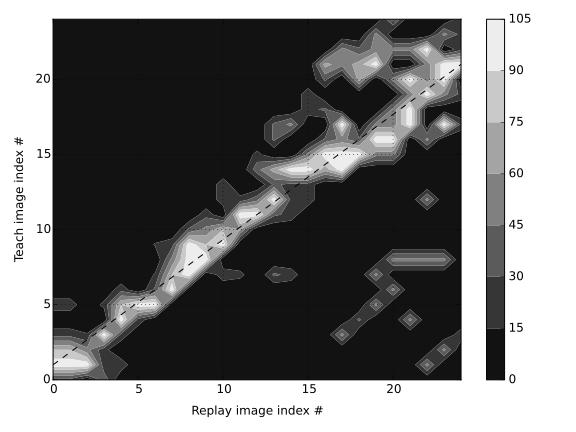
\includegraphics[width=\columnwidth]{indoors_similarity_map.pdf}}\\
\subfloat[Outdoors similarity map]{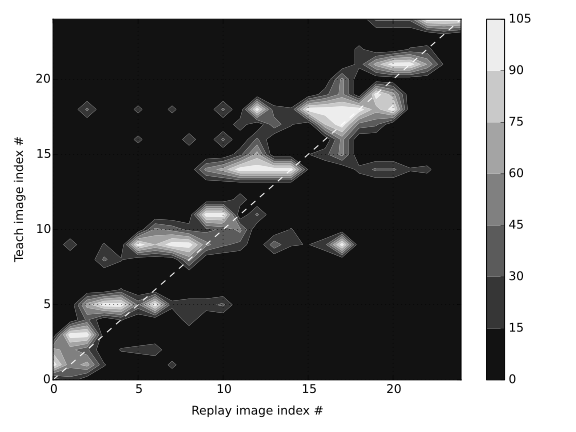
\includegraphics[width=\columnwidth]{outdoors_similarity_map.pdf}}
\caption{Indoors (a) and outdoors (b) similarity maps. Horizontal axis represents replay step images by index number, and the vertical axis, teach step images. Brighter pixels show higher similarity values, and darker pixels, lower similarity. The dashed line indicates the estimated correlation between the image sequences.}
\label{fig:similarity_maps}
\end{figure}

\begin{figure}[t]
\subfloat[Paired replay image]{\includegraphics[width=0.4\columnwidth]{indoors_pairing_replay.eps}}%
\hspace{0.1\columnwidth}%
\subfloat[Paired teach image]{\includegraphics[width=0.4\columnwidth]{indoors_pairing_teach.eps}}
\caption{Example indoors image pair, formed by an image from the replay sequence (a) and matched teach image (b).}
\label{fig:indoors_pair}
\end{figure}

\begin{figure}[t]
\subfloat[Paired replay image]{\includegraphics[width=0.4\columnwidth]{outdoors_pairing_replay.eps}}%
\hspace{0.1\columnwidth}%
\subfloat[Paired teach image]{\includegraphics[width=0.4\columnwidth]{outdoors_pairing_teach.eps}}
\caption{Example outdoors image pair, formed by an image from the replay sequence (a) and matched teach image (b).}
\label{fig:outdoors_pair}
\end{figure}

\begin{figure}[t]
\subfloat[Indoors shift map]{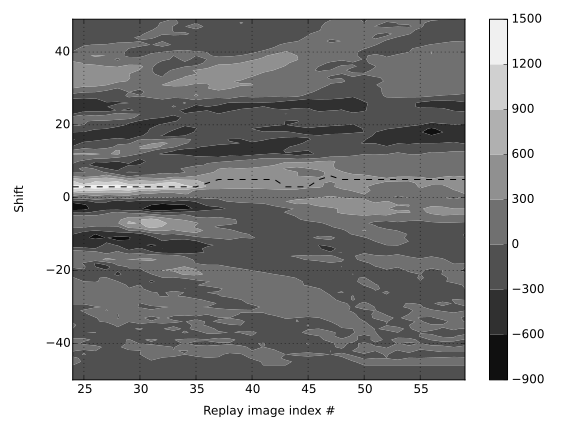
\includegraphics[width=\columnwidth]{indoors_shift_map.pdf}}\\
\subfloat[Outdoors shift map]{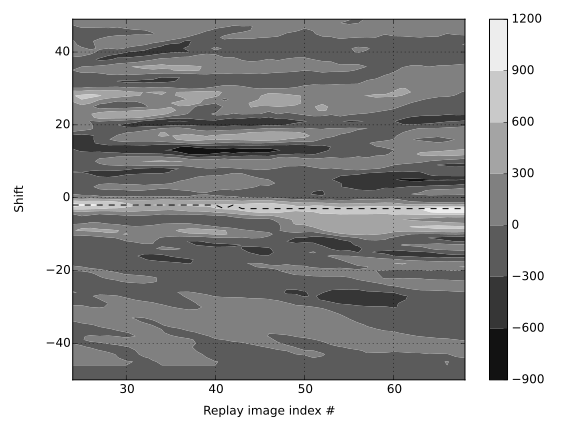
\includegraphics[width=\columnwidth]{outdoors_shift_map.pdf}}
\caption{Shift maps for indoors (a) and outdoors (b) tests. Horizontal axis is replay step image by index number, and vertical axis is shift between teach and replay images -- positive values indicate left shift, and negative values, right. The contour map shows shift likelihood for each replay image across all possible shifts, with brighter pixels representing higher likelihood. A dashed line indicates selected shifts across the replay sequence. The indoors shift map (a) correctly indicates a left shift, consistent with the robot moving leftwards in the replay step relative to the teach step. The outdoors shift map (b) also correctly shows a right shift, consistent with the robot moving rightwards in the replay step relative to the teach step.}
\label{fig:shift_maps}
\end{figure}

A Yamabico robot with a front-mounted camera was set up to perform short trips over straight paths across each environment, collecting video records along the way. These videos, recorded at 20 Frames Per Second (FPS), were later sampled at a rate of 1 FPS to produce the teach and replay image sequences used in the experiments. The image pairing model described in the previous section was implemented on the Open Source C++ library \textbf{Cight}~\cite{HEL14c}, but unfortunately it was not possible to come up with a real-time implementation at this time. Therefore only off-line tests were performed. Method parameters were set to ($\alpha = 30, \beta = 90, z = 10$). The first 25 images of each sequence were used to compute the similarity maps. Initially, a single teach-replay session was recorded at each environment, with linear speed always set to $0.3m/s$.

The indoors environment was deserted when the teach step was recorded, but during the replay step three people came from behind the robot, staying on the right side of the field of view as they walked away; this is reflected in replay images \#30 to \#50. The robot's initial pose in the replay step was turned $2^o$ to the left in relation to the teach step's, but otherwise both steps were recorded from the same start location. Figure~\ref{fig:environments}a-b show samples of these image sequences.

In the outdoors environment a pedestrian came from behind the robot during the teach step, staying on the left side of the visual field as he walked away (this is reflected in teach images \#20 to \#40), but during the replay step there was no one in sight. The robot's initial pose in the replay step was turned $2^o$ to the right in relation to the teach step's, but otherwise both steps were recorded from the same start location. Figure~\ref{fig:environments}c-d show samples of these image sequences.

Figure~\ref{fig:similarity_maps}a shows the similarity map computed for the teach and replay trips recorded in the indoors environment, while Fig.~\ref{fig:similarity_maps}b shows the similarity maps between the outdoors teach and replay trips. The horizontal axis of each similarity map represents replay step images by index number, and the vertical axis, teach step images. Brighter pixels represent higher similarity values, and darker pixels, lower similarity. The dashed line indicates the estimated correlation between the image sequences. Figure~\ref{fig:indoors_pair}a-b and Figure~\ref{fig:outdoors_pair}a-b show a replay image and matched teach image for the indoors and outdoors tests respectively.

In order to assess the adequacy of the computed image pairings for appearance-based navigation, DiVS shift maps~\cite{HEL14d} were computed (with parameters $w = 25, d = 50, e = 5$) on the image pairings defined by the above correlations. Figure~\ref{fig:shift_maps}a shows results for the indoors scenario, and Fig.~\ref{fig:shift_maps}b shows results for the outdoors scenario. For each map horizontal axis is replay step image by index number, and vertical axis is shift between teach and replay images -- positive values indicate left shift, and negative values, right. The contour map shows shift likelihood for each replay image across all possible shifts, with brighter pixels representing higher likelihood. A dashed line indicates selected shifts across the replay sequence. For the indoors test a left shift is correctly reported, consistent with the robot moving leftwards in the replay step relative to the teach step. The outdoors test also correctly reports a shift consistent with the direction of robot motion in the replay step relative to the teach step, in this case to the right.

Additional tests were later recorded in the outdoors environment to assess the method's performance under varying speeds. Three extra replay steps were recorded, from the exactly same initial pose as the teach step, and linear speeds of $0.3m/s$, $0.45m/s$ and $0.6m/s$.

The results for the first test, with linear speed $0.3m/s$, are shown in Figure~\ref{fig:outdoors_30}a-b. Despite a relatively misaligned similarity map, the DiVS shift map correctly reported absent or very small shift, consistent with the replay step following the same path as the teach step. Results for the second test (with linear speed $0.45m/s$) are shown in Figure~\ref{fig:outdoors_45}a-b: in comparison with the first test, the slope of the line over the similarity matrix is much more steep, which is a positive result -- it correctly reflects the faster speed (and hence rate of change in images) of the replay step. The shift map also correctly reports no drift between teach and replay steps.

Results for the last test, with linear speed $0.6m/s$, are somewhat problematic, however. As can be seen in Figure~\ref{fig:outdoors_60}a-b, the slope of the line over the similarity line is \textit{less} steep than in the previous test -- the opposite of what was expected, given the increased speed. Also the DiVS shift map reports a drift to the right, while in fact the robot was again traveling along the same path as the teach step.

\begin{figure}[t]
\subfloat[Similarity map]{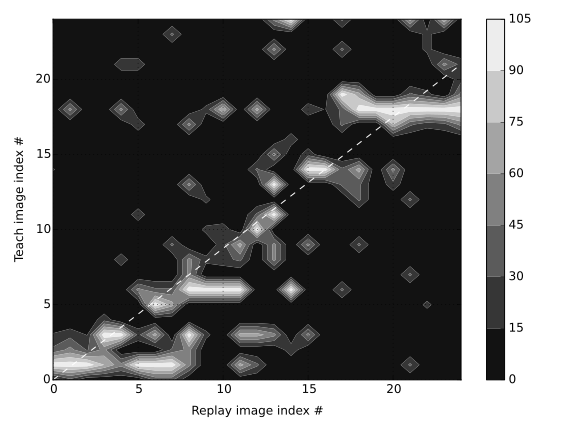
\includegraphics[width=\columnwidth]{outdoors_similarity_map_30.pdf}}\\
\subfloat[Shift map]{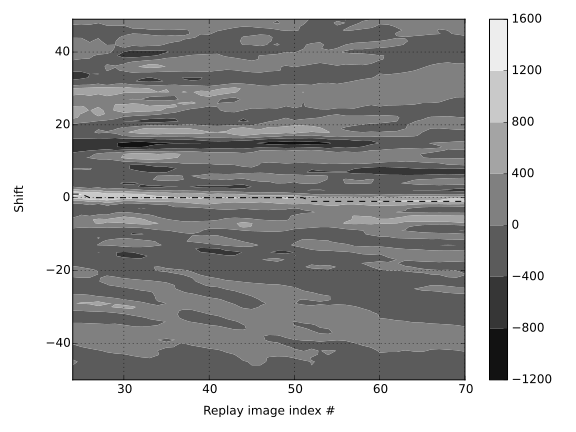
\includegraphics[width=\columnwidth]{outdoors_shift_map_30.pdf}}
\caption{Later outdoors test with identical initial poses for teach and replay steps. Linear speed was set to $0.3m/s$ at both steps. In the similarity map, horizontal axis represents replay step images by index number, and the vertical axis, teach step images. Brighter pixels show higher similarity values, and darker pixels, lower similarity. The dashed line indicates the estimated correlation between the image sequences. In the shift map, horizontal axis is replay step image by index number, and vertical axis is shift between teach and replay images -- positive values indicate left shift, and negative values, right. The contour map shows shift likelihood for each replay image across all possible shifts, with brighter pixels representing higher likelihood. A dashed line indicates selected shifts across the replay sequence. Despite a relatively misaligned similarity map, the shift map correctly reports absent or very small shift, consistent with the replay step following the same path as the teach step.}
\label{fig:outdoors_30}
\end{figure}

\begin{figure}[t]
\subfloat[Similarity map]{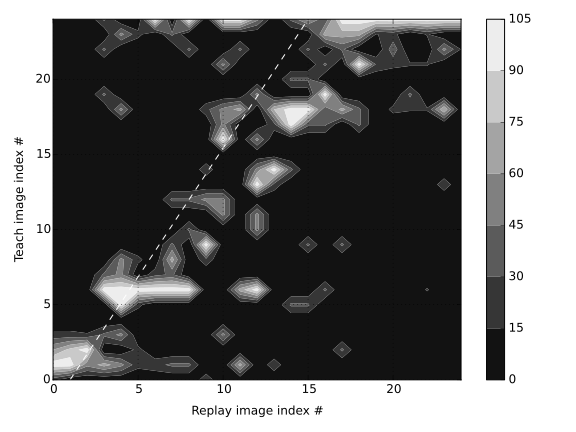
\includegraphics[width=\columnwidth]{outdoors_similarity_map_45.pdf}}\\
\subfloat[Shift map]{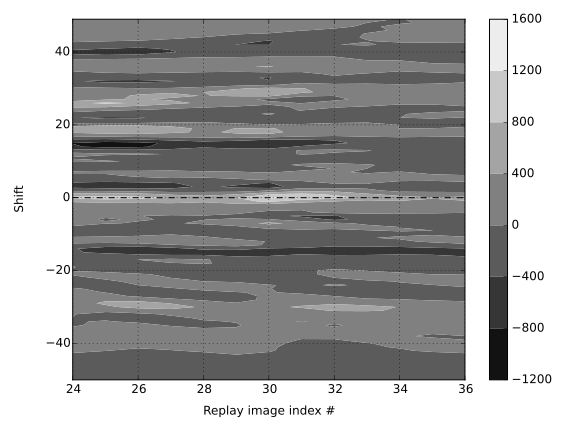
\includegraphics[width=\columnwidth]{outdoors_shift_map_45.pdf}}
\caption{Outdoors test with identical initial poses for teach and replay steps. Linear speed was set to $0.3m/s$ at the teach step, and $0.45m/s$ at the replay step. In the similarity map, horizontal axis represents replay step images by index number, and the vertical axis, teach step images. Brighter pixels show higher similarity values, and darker pixels, lower similarity. The dashed line indicates the estimated correlation between the image sequences. In the shift map, horizontal axis is replay step image by index number, and vertical axis is shift between teach and replay images -- positive values indicate left shift, and negative values, right. The contour map shows shift likelihood for each replay image across all possible shifts, with brighter pixels representing higher likelihood. A dashed line indicates selected shifts across the replay sequence. In comparison with the first test, the slope of the line over the similarity matrix is much more steep, which is a positive result -- it correctly reflects the faster speed (and hence rate of change in images) of the replay step. The shift map also correctly reports no drift between teach and replay steps.}
\label{fig:outdoors_45}
\end{figure}

\begin{figure}[t]
\subfloat[Similarity map]{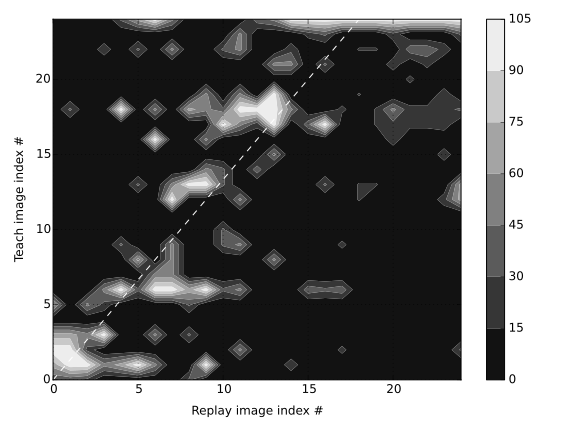
\includegraphics[width=\columnwidth]{outdoors_similarity_map_60.pdf}}\\
\subfloat[Shift map]{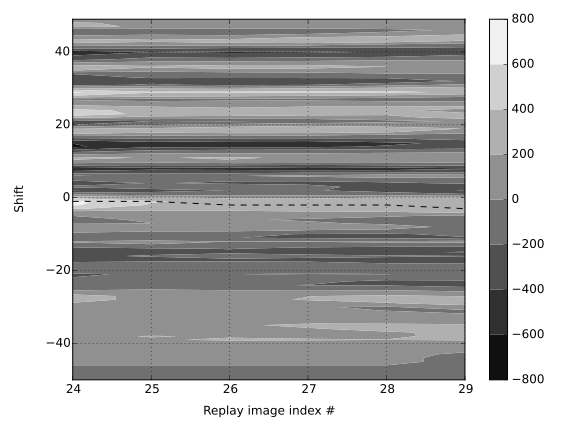
\includegraphics[width=\columnwidth]{outdoors_shift_map_60.pdf}}
\caption{Outdoors test with identical initial poses for teach and replay steps. Linear speed was set to $0.3m/s$ at the teach step, and $0.6m/s$ at the replay step. In the similarity map, horizontal axis represents replay step images by index number, and the vertical axis, teach step images. Brighter pixels show higher similarity values, and darker pixels, lower similarity. The dashed line indicates the estimated correlation between the image sequences. In the shift map, horizontal axis is replay step image by index number, and vertical axis is shift between teach and replay images -- positive values indicate left shift, and negative values, right. The contour map shows shift likelihood for each replay image across all possible shifts, with brighter pixels representing higher likelihood. A dashed line indicates selected shifts across the replay sequence. The slope of the line over the similarity line is \textit{less} steep than in the previous test -- the opposite of what was expected, given the increased speed. Also the DiVS shift map reports a drift to the right, while in fact the robot was again traveling along the same path as the teach step.}
\label{fig:outdoors_60}
\end{figure}

\section{Conclusion}

This article presented \textit{feature point correlation}, a method for pairing images from different sequences collected over successive trips along the same route. Image pairings are shown to correlate well with viewpoint proximity, which is a useful feature for appearance-based navigation systems. Tests performed under different environments demonstrate the method's robustness. Moreover, tests employing DiVS shift computation show the computed pairings to be fit for practical use.

Currently the method's main weakness is the time it takes to compute a similarity matrix, in the order of $30s$ for a matrix as small as $25 \times 25$. Several measures can be taken to improve performance though, such as restricting matrix computation to a sparse image set (so only a handful of characteristic images are inspected), optimizing feature selection (so within each image only a handful of high-quality feature points are inspected), and parallel feature inspection. Accordingly, more reliable image mapping, feature selection and line fitting methods could also be researched.

\footnotesize

\bibliographystyle{IEEEtran}
\bibliography{references}

\normalsize

\end{document}
